\input{wg21common}

% Footnotes at bottom of page:
 \usepackage[bottom]{footmisc} 

% Table going across a page: 
 \usepackage{longtable}

 % Start sections at 0
% \setcounter{section}{-1}

% color boxes
\usepackage{tikz,lipsum,lmodern}
\usepackage[most]{tcolorbox}

%%%%%%%%%%%%%%%%%%%%%%%%%%%%%%%%%%%%%%%%%%%%%%%%

%TABLE OF CONTENTS SETTINGS

\usepackage{titlesec}
\usepackage{tocloft}

% Custom ToC layout because the default sucks
\cftsetindents{section}{0in}{0.24in}
\cftsetindents{subsection}{0.24in}{0.34in}
\cftsetindents{subsubsection}{0.58in}{0.44in}

% Needed later to reduce the ToC depth mid document
\newcommand{\changelocaltocdepth}[1]{%
  \addtocontents{toc}{\protect\setcounter{tocdepth}{#1}}%
  \setcounter{tocdepth}{#1}%
}

\setcounter{tocdepth}{3}

%%%%%%%%%%%%%%%%%%%%%%%%%%%%%%%%%%%%%%%%%%%%%%%%

\begin{document}
\title{Contract assertions on function pointers}
\author{ Timur Doumler \small(\href{mailto:papers@timur.audio}{papers@timur.audio}) 
}
\date{}
\maketitle

\begin{tabular}{ll}
Document \#: & D3327R0 \\
Date: &2024-10-05 \\
Project: & Programming Language C++ \\
Audience: & SG21, EWG
\end{tabular}

\begin{abstract}
In this paper, we explore the design space for an extension to the Contracts MVP proposal \cite{P2900R8} that would allow placing function contract assertions --- \tcode{pre} and \tcode{post} --- directly on pointers to functions and pointers to member functions. We begin  with a summary of the prior art in this design space. We list different use cases for such a feature. We then discuss the available \emph{syntactic} space. Finally, we discuss different  options for the compile-time and runtime \emph{semantics} of this feature, as well as possible specification strategies and their tradeoffs and limitations.
\end{abstract}

%%%%%%%%%%%%%%%%%%%%%%%%%%%%%%%%%%%%%%%%%%%%%

\tableofcontents*
\pagebreak

%\section*{Revision history}

%Revision 0 (2024-04-16)
%\begin{itemize}
%\item Original version
%\end{itemize}

%\pagebreak

%%%%%%%%%%%%%%%%%%%%%%%%%%%%%%%%%%%%%%%%%%%%%

\section{Introduction}
\label{intro}

Indirect function calls through function pointers remain a staple of software interface design and implementation in C++, and of pervasive use. Consequently, it seems desirable that the Contracts MVP proposal \cite{P2900R8} supports efficient use of contract assertions with function pointers. As a possible use case, consider an API that relies on function pointers, for example a driver API for interacting with a hardware device:
\begin{codeblock}
typedef int32_t (*device_io_ptr)(void*, uint8_t, uint8_t*);
struct device_io_t {
  device_io_ptr device_read;
  device_io_ptr device_write;
  // ...
};
\end{codeblock}
To detect and mitigate possible misuse of such an API, it would be desirable to attach function contract assertions --- \tcode{pre} and \tcode{post} --- directly to the function pointers in order to add contract checks to the function calls made through them. Such checks can verify preconditions on the passed-in parameters, postconditions on the returned values, and potentially other parts of the API's contract.

The need for such a feature has been recognised, and named by a major compiler vendor as a criterion for whether the Contracts MVP is indeed viable. However, despite the interest in such a feature, no proposal that would allow placing \tcode{pre} and \tcode{post} directly on pointers to functions and pointers to member functions has been published to date. This paper does not contain such a proposal, either. Rather, the purpose of this paper is to explore the design space for such a proposal and to discuss the challenges and open questions that any such proposal must address.

The paper is structured as follows. In Section \ref{priorart}, we summarise the prior art in this design space --- how past C++ Contracts proposals have dealt with the question of contract assertions on function pointers, and what papers have been published in this design space more recently. In Section \ref{usecases}, we consider various possible use cases for attaching \tcode{pre} and \tcode{post} directly on function pointers. In Section \ref{syntax}, we explore the available syntactic space for such an extension. In Section \ref{semantics}, we explore different options for the compile-time and runtime semantics: when working with \tcode{pre} and \tcode{post} on function pointers, when should the program compile, when should it not, and what should its behaviour be --- in particular, when calling through a function pointer, which contracts should be checked when? Finally, in Section \ref{wherelive}, we analyse three possible strategies for specifying such a feature, and their respective tradeoffs and limitations. We discuss where and how a contract assertion sequence attached to a function pointer should be stored --- as part of the pointer's type, as part of its value, or as a property of the variable declaration?

In the immediate future, the question needs to be answered whether the Contracts MVP proposal \cite{P2900R8} should be delayed until we have a consensus solution to the problem of contract assertions on function pointers, or whether it is acceptable to ship the Contracts MVP without such a feature and instead add it as a post-MVP extension at a later time. We do not attempt to give an answer here, but we hope that the material in this paper will inform that discussion.

%%%%%%%%%%%%%%%%%%%%%%%%%%%%%%%%%%%%%%%%%%%%%

\section{Prior art}
\label{priorart}

A first exploration of placing contract assertions on function pointers --- including many of the thoughts we explored in more depth here --- can be found in \cite{N4110}. The paper draws the conclusion that making these assertions part of the type system is not a viable solution. The idea to make the contract a property of the declaration instead first appears in  \cite{P0246R0} and \cite{P0247R0}.

The first concrete proposal for placing contract assertions on function pointers can be found in a series of papers from the early C++2a Contracts era: \cite{N4415}, \cite{P0287R0}, and \cite{P0380R0}. In these papers, contract assertions could be placed directly on function pointers, but assigning a function to such a pointer, or assigning the value of a pointer to function to another such pointer, was ill-formed unless the function contract assertions on both entities match. The contract assertions were neither a part of the type nor a part of the pointer value. The problem of how to propagate contract information from typedefs (see \ref{propagation}) was recognised but not solved in these papers:  if a typedef is used to declare a function type or a pointer to function type, any contracts in the typedef declaration would not transfer to the function or to the pointer.

The motivation given in those papers for this approach was to guarantee that when a function is called through a pointer, its function contract assertions are still checked. However, in revision \cite{P0380R1} it was realised that there is a much more effective way to achieve this, without placing undue burden on the user: we can specify that when a function is called through a pointer, its own function contract assertions are still evaluated as if it was called directly. This effectively introduced what we now call caller-facing and callee-facing contracts, with the limitation that the callee-facing contract of a function pointer is empty (or, to be more precise, cannot yet be specified with function contract assertions). At that point, the idea to place \tcode{pre} and \tcode{post} directly on function pointers was abandoned and made ill-formed. This carried over into the Contracts C++2a proposal \cite{P0542R5} and ultimately into today's Contracts MVP \cite{P2900R8}, where it is now the status quo.

In \cite{P3173R0}, a major compiler vendor stated that a Contracts facility that fails to adequately support efficient use with pointer to functions is woefully inadequate and unready for prime use. At the WG21 meeting in Tokyo (February 2023), where that paper was discussed, an EWG poll showed significant interest in such a feature, although there was no consensus that it must be included in a Contracts MVP (see \cite{P3197R0}).

No concrete proposal to add \tcode{pre} and \tcode{post} to function pointers followed, but two papers proposed to carve out design space in the Contracts MVP for adding such a feature as a later extension. \cite{P3221R0} proposed making taking the address of a function with function contract assertions ill-formed, while \cite{P3250R0} proposed to make it ill-formed to deduce the type of such a function. Both proposals were rejected by SG21.

The latest proposal in this space at the time of writing is \cite{P3271R0}. It does \emph{not} propose to allow attaching \tcode{pre} and \tcode{post} to function pointers directly (the approach that we explore in this paper). Instead, it introduces so-called \emph{function usage types}, along with new syntax to define them:
\begin{codeblock}
int takes_and_returns_positive_numbers(int i) usage 
  pre (i > 0)
  post (r: r > 0);
\end{codeblock}
We can then declare a pointer to such a function usage type, assign the address of a function to that pointer, and call the function through that pointer, which will perform a check of the usage type's contract around that call.

In this model, function usage types are a distinct kind of types different from function pointer types, and two function usage type that differ only in their contract assertion sequence are different types. Simultaneously, a function usage type is a type that is \emph{similar} to the corresponding function pointer type without a contract assertion sequence (e.g., \tcode{int} and \tcode{const int} are \emph{similar} types; so are \tcode{int[3]} and \tcode{int[]}). This means essentially that both types have the same value representation and are thus ABI-compatible.

The approach in \cite{P3271R0} combines some of the advantages of the type system approach (see \ref{type}), such as being compatible with templates and type deduction, with the advantages of the ``property of the declaration'' approach (see \ref{decl}), such as no impact on ABI and no breakage of client code. However, it introduces a novel kind of entity to the language instead of allowing to attach \tcode{pre} and \tcode{post} directly on function pointers as they exist in C++ today. This might or might not turn out to be a viable solution to the problem. In this paper, we do not consider solutions that introduce a new novel of entity instead of using function pointers directly. In this sense, our paper can be considered complementary material to \cite{P3271R0}.

%%%%%%%%%%%%%%%%%%%%%%%%%%%%%%%%%%%%%%%%%%%%%
\section{Use cases}
\label{usecases}

In this section, we list some known \emph{use cases} that can serve as motivation for an extension to \cite{P2900R8} that allows \tcode{pre} and \tcode{post} on function pointers. Some of these use cases may be more plausible than others, and some may have contradicting requirements; here, we limit ourselves to describing them, with no attempt at judging or prioritising.

\subsection{Enable caller-side checking of contracts not visible at the call site}
\label{usecase_ville}

One possible use case for \tcode{pre} and \tcode{post} on function pointers is to introduce a mechanism to make the function contract assertions of a function visible in a context that does not see the declaration of that function, because which function will be called is being determined elsewhere at runtime. In particular, this can enable caller-side checking of a function's contract in contexts where this is currently not possible with \cite{P2900R8}.

Consider:
\begin{codeblock}
int f(int x) pre(x >= 0);
int g(void (*fptr)(int x) pre (int x >=0)); // definition in another TU

void using_code() {
   int (*fptr)(int x) pre(x >= 0) = f;
   g(fptr);
}
\end{codeblock}
In this scenario, the definition of \tcode{g} might not know that the function that ends up being called is \tcode{f}, and might not see its declaration and therefore its sequence of function contract assertions. However, by using the pointer \tcode{fptr} that has a matching sequence of function contract assertions, the compiler is able to perform caller-side checking of \tcode{f}'s function contract assertions inside the definition of \tcode{g}.

%---------------------------------------------------------------------------------------------------------------------

\subsection{Add a missing function contract check}
\label{usecase_addmissing}

Another possible use case for \tcode{pre} and \tcode{post} on function pointers is to add contract checks to an existing function where the declaration of that function cannot be changed for whatever reason:
\begin{codeblock}
// legacy function; the behaviour is undefined if \tcode{x < 0}
int f(int x);   

int (*f_checked)(int x) pre (x >= 0) = f; 

void using_code() {
  f(-3);          // unsafe call to \tcode{f}
  f_checked(-3);  // safe call to \tcode{f} if contract checks are enabled
}
\end{codeblock}

Note that the same effect can already be achieved with \cite{P2900R8} without involving function pointers. If we cannot modify the declaration of \tcode{f}, but we can modify the definition, we can add the desired precondition check with a \tcode{contract_assert} statement at the start of the function body. If we cannot modify the declaration either, we can wrap \tcode{f} with another function or a lambda that has the desired precondition check:
\begin{codeblock}
auto f_checked = [](int x) pre (x >= 0) { return f(x); }
\end{codeblock}
Note that such a captureless lambda implicitly converts to a function pointer.

%---------------------------------------------------------------------------------------------------------------------

\subsection{Augment function-pointer-based APIs with contract checks}
\label{usecase_api}

There exist numerous C and C++ APIs that make use of function pointers. Consider, for example, the following code that uses a callback API:
\begin{codeblock}
// library code
typedef int(*callback_t)(int);
void register_callback(callback_t);

// application code
int f(int i); 
int main() {
  register_callback(f);
  // ...
}
\end{codeblock}
Now, we might want to augment this callback API with contract assertions. For example, the  API might ensure that no negative numbers are passed into the callback, and expect that no negative numbers are returned from it. We might want to express those preconditions and postconditions directly on the API:
\begin{codeblock}
typedef int(*callback_t)(int i) 
  pre (i >= 0) 
  post (r: r >= 0);
  
void register_callback(callback_t);
  
int f(int i);  // no \tcode{pre} and \tcode{post} here
int main() {
  register_callback(f);  // contract will be checked when callback is called
  // ...
}
\end{codeblock}
Instead of a callback API, we could also be dealing with a struct-based API like the one from Section~\ref{intro}:
\begin{codeblock}
typedef int32_t (*device_io_ptr)(void*, uint8_t, uint8_t*);
struct device_io_t {
  device_io_ptr device_read;
  device_io_ptr device_write;
  // ...
};
\end{codeblock}
Again, we might want to express preconditions and postconditions on the involved function pointers directly on the API:
\begin{codeblock}
typedef int32_t (*device_io_ptr)(void* device_ptr, uint8_t in, uint8_t* out)
  pre (device_ptr != nullptr)
  pre (out != nullptr)
  post (r: r >= 0);
  
\end{codeblock}
In each case, we want to be able to enable checks of the API's contract to detect and mitigate misuse. Depending on the shape of the API, we might want to attach the contract assertions either to a typedef that is later used to declare parameters and data members of type pointer to function, or to the declarations of those parameters and data members directly.
\subsection{Check function contracts when using function-pointer-based legacy APIs}
\label{usecase_legacyapi}

We might be dealing with legacy function pointer based APIs which look like the one in the previous example but cannot be changed for whatever reason, so we cannot add \tcode{pre} and \tcode{post} to the API itself. Instead, we might want to add \tcode{pre} and \tcode{post} to the function passed in. If contract checks are enabled, we want those assertions to be checked even if the API is entirely unaware of them as the function pointer itself does not have any function contract assertions:
\begin{codeblock}
// library code --- legacy API
typedef int(*callback_t)(int);
void register_callback(callback_t);

// application code
int f(int i) pre (i >= 0) post (r: r >= 0); 
int main() {
  register_callback(f);  // contract will be checked when callback is called
  // ...
}
\end{codeblock}
Note that this use case is already satisfied by \cite{P2900R8} today: if calling a function \tcode{f} with function contract assertions, those assertions are guaranteed to be evaluated even if \tcode{f} is called through a function pointer that does not have any contract assertions attached to it. We might want to preserve this functionality when adding an extension that allows \tcode{pre} and \tcode{post} on function pointers.

%---------------------------------------------------------------------------------------------------------------------

\subsection{Inject a contract check via a function pointer}
\label{usecase_inject}
Consider again the legacy callback API from the previous use case. A more complicated scenario can occur where not only the API itself, but also the passed-in callback \tcode{f} cannot be modified to add \tcode{pre} and \tcode{post}. In this case, we might want to inject the contract via an intermediate pointer, and expect that the contract does not get lost when that pointer is passed to the legacy API:
\begin{codeblock}
// library code --- legacy API
typedef int(*callback_t)(int);
void register_callback(callback_t);

// application code
int f(int i); 
int main() {
  int (*f_checked)(int i) pre (i >= 0) post (r: r >= 0) = f;
  register_callback(f_checked);  // contract should be checked when callback is called
  // ...
}
\end{codeblock}
Note that this is a variation of use case \ref{usecase_addmissing}, but the pointer with \tcode{pre} and \tcode{post} is now being assigned to \emph{another} pointer \emph{without} matching \tcode{pre} and \tcode{post}. Again, this functionality can be achieved with \cite{P2900R8} today by using a captureless lambda wrapper instead of an intermediate function pointer.

%---------------------------------------------------------------------------------------------------------------------

\subsection{Augment APIs with caller-facing checks in addition to callee-facing checks}
\label{usecase_callercallee}
As an extension of use case \ref{usecase_api}, we might want to add \tcode{pre} and \tcode{post} to a function pointer to express a \emph{caller-facing} contract, which is checked independently from --- and in addition to --- the \emph{callee-facing} contract, which is the contract on the declaration of the function that the pointer points to.

Consider for example some numerical algorithm \tcode{crunchNumbers} that takes a pointer to function and has a precondition that this function, when called, only returns positive numbers. We might want to express this contract directly on that pointer:
\begin{codeblock}
void crunchNumbers(int(*positiveGenerator)() post (r : r > 0)) {
  // do stuff with positive numbers returned by \tcode{positiveGenerator}...
}
\end{codeblock}
Now, we might pass different functions into \tcode{crunchNumbers}, which might do different things, and therefore have their own, distinct contracts:
\begin{codeblock}
// This function produces only multiples of three
int f1() post (r: r % 3 == 0);

// This function produces only prime numbers
int f2() post (r: isPrime(r));

// etc.
\end{codeblock}
Now, if we pass \tcode{f1}, \tcode{f2}, etc. into \tcode{crunchNumbers}, we might want both sets of contract assertions to be checked.

Note that for this use case, these sets are conceptually completely independent from each other. The functions \tcode{f1}, \tcode{f2}, etc. might not guarantee, in general, that the number returned is always positive (it is not part of their contract); however, \tcode{crunchNumbers} must call those functions only in ways where they end up producing positive numbers (because it is part of its contact). Otherwise, a contract violation will occur, indicating a failure to combine the different program components correctly.

%---------------------------------------------------------------------------------------------------------------------

\subsection{Use in templates}
\label{usecase_templates}
Finally, we might want to add contract checks in templates, and pass user-defined function contract assertions to such templates. For example, we might want to define a \tcode{std::function} that has particular contract assertions attached to its call operator, or a \tcode{std::vector} of function pointers that all have a particular sequence of contract assertions attached to them:
\begin{codeblock}
// Pointer to function that expects a nonnegative integer:
typedef int (*nonnegative_fptr_t)(int i) pre (i >= 0);

std::function<nonnegative_fptr_t> my_nonnegative_func;
std::vector<nonnegative_fptr_t>   my_nonnegative_funcs;
// etc.
\end{codeblock}
This should work correctly with template argument deduction and class template argument deduction as well:
\begin{codeblock}
nonnegative_fptr_t fptr = f;

void test(int i) {
  // Template argument deduction:
  std::invoke(fptr, i);
  
  // Class template argument deduction:
  std::function my_nonnegative_func(fptr);
  my_nonnegative_func(i);
}
\end{codeblock}
When the underlying function is invoked inside a function template (\tcode{std::invoke}, \tcode{std::sort}, ...), invoked inside a class template's call operator (\tcode{std::function}), invoked inside some other member function of a class template (comparator in \tcode{std::set}, \tcode{std::map}, ...), or retrieved from a container and then invoked by the user (\tcode{std::vector}, ...), the expectation is that the function contact assertions of the function should be evaluated.


%%%%%%%%%%%%%%%%%%%%%%%%%%%%%%%%%%%%%%%%%%%%%

\section{Syntax}
\label{syntax}

If we want to attach \tcode{pre} and \tcode{post} to function pointers, we need to understand how and in which contexts we can spell that, and whether such a syntax could be added as an extension of the existing contracts syntax in \cite{P2900R8}.

\subsection{Contract assertions on declarations}

In the \cite{P2900R8} grammar, the sequence of \tcode{pre} and \tcode{post} specifiers attached to the declaration of a function or lambda is represented by the grammar production \emph{function-contract-specifier-seq}. The grammar allows for a \emph{function-contract-specifier-seq} to be attached to any \emph{abstract-declarator}. Therefore, an extension to \cite{P2900R8} is feasible that allows attaching \tcode{pre} and \tcode{post} to the declaration of a variable of type pointer to function or pointer to member function:
\begin{codeblock}
int (*nonnegative_fptr)(int i) pre (i >= 0);        // OK
int (*X::nonnegative_memfptr)(int i) pre (i >= 0);  // OK
\end{codeblock}
It is also syntactically possible to attach \tcode{pre} and \tcode{post} to a typedef or using declaration:
\begin{codeblock}
typedef int (*nonnegative_fptr_t)(int i) pre (i >= 0);  // OK
using nonnegative_fptr_t = int(*)(int i) pre (i >= 0);  // OK
\end{codeblock}
Now, if we declare a pointer variable using one of the above typedefs, we need to choose whether the  \tcode{pre} and \tcode{post} should be attached to the typedef or to the variable declaration. The latter seems less useful as it would be impossible to use function parameters inside the predicate:
\begin{codeblock}
typedef int (*nonnegative_fptr_t)(int i) pre (i >= 0);  
nonnegative_ftpr_t my_fptr;  // OK; pointer with precondition

typedef int (*fptr_t)(int i);
fptr_t my_fptr pre (/* ??? */);  // cannot name \tcode{i} here
\end{codeblock}

\subsection{Contract assertions on typenames}

With the \cite{P2900R8} grammar it is impossible to attach a \emph{function-contract-specifier-seq} to a \emph{type-identifier}; an attempt to do so would result in parsing ambiguities. This means that we cannot specify an extension that would allow attaching \tcode{pre} and \tcode{post} directly to the return type of a function:
\begin{codeblock}
int (*ftpr)(int i) pre (i >= 0) get_nonnegative_fptr();  // Error; \tcode{pre} parsed as function name
\end{codeblock}
Instead, we would have to use a typedef:
\begin{codeblock}
typedef int (*nonnegative_fptr_t)(int i) pre (i >= 0); 
nonnegative_fptr_t get_nonnegative_fptr();  // OK
\end{codeblock}
Similarly, it would not be possible to attach \tcode{pre} and \tcode{post} directly to the typename when casting to a function pointer type with  \tcode{pre} and \tcode{post}, when using a function pointer type with \tcode{pre} and \tcode{post} as a template argument, or in other contexts where a function pointer type appears outside of a declarator.

In all of these cases, the desired construction can be expressed syntactically with the help of a typedef. This limitation seems acceptable; to remove it, we would have to adopt an entirely different syntax for contracts. We do not explore options for an entirely different contracts syntax further in this paper, but we do note that placing contract assertions on function types (and therefore also on function pointer types) seems possible\footnote{This has been pointed out in \cite{P2935R4} and \cite{P3028R0}. Nevertheless,  placing contract assertions on function types has not been considered by SG21 as one of the requirements for choosing an appropriate contracts syntax; it is not listed in \cite{P2885R3}, which served as the basis for choosing the syntax proposed in \cite{P2961R2} for the Contracts MVP. A possible explanation is that the idea was not well understood at the time.} with the attribute-like syntax of C++2a Contracts \cite{P0542R5}. 

\subsection{Contract assertions on expressions}
\label{syntax_expr}

Finally, we could consider attaching \tcode{pre} and \tcode{post} to an expression of type pointer to function or pointer to member function. For example, consider a call expression that evaluates to a function pointer which is then itself called:

\begin{codeblock}
int (*)(int) get_fptr();

void test(int i) {
  get_fptr()(i);
}
\end{codeblock}
We might want to attach \tcode{pre} and \tcode{post} directly to the prvalue \tcode{get_fptr()}. The \cite{P2900R8} grammar does not allow this; neither does any other known proposal for a contracts syntax. In general, this seems unlikely to be feasible, considering the compexity of the C++ expression grammar and the fact that even attributes --- which are syntactically clearly separated from other constructs --- cannot appertain to expressions, only to entities and statements.

%%%%%%%%%%%%%%%%%%%%%%%%%%%%%%%%%%%%%%%%%%%%%

\section{Semantics}
\label{semantics}

If we want to allow \tcode{pre} and \tcode{post} on function pointers, we need to define what should happen when we initialise a function pointer variable with the address of a function, assign the address of a function to that variable, pass a function pointer into a function as a parameter, return a function pointer from a function, and evaluate arbitrary expressions involving function pointers, in a world where any function or function pointer involved in the expression could have an arbitrary sequence of function contract assertions attached to it.

We need to specify the compile-time semantics of such operations --- which combinations should be well-formed? --- as well as the runtime behaviour of a call through the resulting pointer --- which contracts should be checked during such a call? In this section, we discuss the known options.

%---------------------------------------------------------------------------------------------------------------------

\subsection{Pointer contract matches function contract}
\label{matching}

The simplest case is that of assigning (or initialising with, passing, returning, etc.) the address of a function with a particular contract assertion sequence to a function pointer declared with the same contract assertion sequence. 
\begin{codeblock}
int f(int i) pre (i >= 0);
int (*fptr)(int i) pre (i >= 0);

void test(int i) {
  fptr = f; 
  fptr(i); 
}
\end{codeblock}
The only reasonable expectation seems to be that the above code should ``just work'' and that the precondition assertion \tcode{pre (i >= 0)} should be evaluated when calling \tcode{f} through \tcode{fptr}.

While it seems clear that the above code should be \emph{allowed}, and has unambiguous semantics, it is worth asking the question whether we should \emph{require} the contract assertion sequence of the pointer to match that of the function. This would be the direction that was proposed in \cite{N4415}, \cite{P0287R0}, and \cite{P0380R0}, before being abandoned in later Contracts proposals (see Section~\ref{priorart}).

Requiring the contract assertion sequences to match satisfies use case \ref{usecase_ville}. However, note that when two functions do \emph{different things}, they will typically have different contracts, even if they have the same signature (consider for example a function that computes the square root of a number and one that computes the cubic root). There are situations where two distinct functions have the same contract, but we do not expect this to be the common case. One example would be a group of functions that all do the same same thing \emph{in a different way}, for example functions implementing different numeric algorithms to compute the square root that all offer the same guarantees. If we require the contract assertion sequences to match, we effectively restrict function pointers to always point to a function from one such group, or at least limit the subset of the contract that can be expressed with function contract assertions (rather than in plain language) to the common subset of all functions that the given pointer could point to.

Another concern with requiring the contract assertion sequences to match is that we would need to ensure that it is impossible to SFINAE on whether two entities have the same contract assertion sequence. Failure to do so would violate the Contracts Prime Directive\footnote{The \emph{Contracts Prime Directive} stipulates that the mere addition of a contract assertion should never alter the semantics of a correct program, and therefore should not be visible to concepts, SFINAE, overload resolution, the \tcode{noexcept} operator, and other forms of compile-time branching. However, if adding \tcode{pre} and \tcode{post} to a function can change its type, it would directly violate that principle.} from \cite{P2900R8} and impede future extensions that relax this requirement.

Note that \cite{P2900R8} does not specify how many times any given contract assertion will be evaluated. Therefore, for the semantics of the code above it does not matter whether we choose a design where the precondition assertions on \tcode{f} and \tcode{fptr} are distinct and independent, or one where they are required to be the same.

%---------------------------------------------------------------------------------------------------------------------

\subsection{Pointer drops function contract}
\label{dropping}

The next case is that of assigning the address of a function with a particular function contract assertion sequence to a function pointer that does not have \emph{any} such assertions attached to it:
\begin{codeblock}
int f(int i) pre (i >= 0);
int (*fptr)(int i);

void test(int i) {
  fptr = f; 
  fptr(i); 
}
\end{codeblock}
For this case, we have multiple possibilities. We could make the assignment ill-formed, which would satisfy use case \ref{usecase_ville} but be a breaking change to \cite{P2900R8}, where the above code is valid today, or we could continue to allow it.

If we allow it, the question is whether the call through \tcode{fptr} would evaluate the precondition assertion of \tcode{f} or not. Evaluating the precondition assertion seems to be the only sensible answer: if the function \tcode{f} has function contract assertions, the expectation is that those assertions will be evaluated if that function is called, regardless of whether that happens through a pointer or otherwise. A consequence is that the value of the pointer \tcode{fptr} --- without any contract assertions attached to it --- could be passed into a function, returned from a function, be the result of evaluating an expression, etc. In all cases, the function contract assertions of \tcode{f} would be checked when calling it through the resulting pointer. This is the behaviour in \cite{P2900R8} today and is required to satisfy use case \ref{usecase_legacyapi}.

%---------------------------------------------------------------------------------------------------------------------

\subsection{Pointer adds contract}
\label{adding}

The inverse of the previous case is assigning the address of a function that does \emph{not} have any function contract assertions to a function pointer that does:
\begin{codeblock}
int f(int i);
int (*fptr)(int i)  pre (i >= 0);

void test(int i) {
  fptr = f;
  fptr(i); 
}
\end{codeblock}
With \cite{P2900R8} today, the code above does not compile as \tcode{pre} and \tcode{post} on function pointers are not allowed. If we were to allow them, we need to decide whether the assignment should compile, and whether the call through \tcode{fptr} should evaluate the precondition assertion of \tcode{fptr}.

Making the assignment ill-formed would satisfy use case \ref{usecase_ville}. If we allow the assignment, the only sensible answer for the runtime behaviour of the call seems to be that the precondition assertion of \tcode{fptr} should be evaluated: why would we write contract assertions on a pointer if they are not evaluated when using that pointer? This behaviour would enable use case \ref{usecase_addmissing}.

If we go down this route, then it seems that contract assertions on a parameter declaration should also be checked when calling a function through that parameter:
\begin{codeblock}
int f(int i);

void invoke_ptr(int (*fptr)(int i) pre (i >= 0), int i) {
  fptr(i);
}

void test(int i) {
  invoke_ptr(f, i);
}
\end{codeblock}
This behaviour would enable use case \ref{usecase_api}.

One implication of this direction is that the contract assertions on a function pointer are now inevitably unique to \emph{that} pointer, and therefore must be stored together with the pointer somehow --- either as part of its type, or as part of its value, or as a property of the pointer variable declaration; each choice comes with  tradeoffs and limitations (see Section~\ref{wherelive}).
 
%------------------------------------------------------------------------------------------------------

\subsection{Pointer contract is different from function contract}
\label{ptrfundifferent}

Now, let us consider the case of assigning the address of a function with a sequence of function contract assertions to a function pointer \tcode{fptr} that has a \emph{different} sequence of contract assertions (we could construct an analogous test case for initialising a function pointer variable, or passing a function address into a function taking a function pointer as a parameter):
\begin{codeblock}
int f(int i)
  pre (i % 2 == 0)      // must call with even integer
  post (r: r % 2 == 0); // guaranteed to return even integer

int (*fptr)(int i)
  pre (i > 0)           // must call with positive integer
  post (r: r != 0);     // guaranteed to return non-zero integer

void test(int i) {
  fptr = f; 
  fptr(i);   
}
\end{codeblock}
The example above shows assignment to a function pointer variable. Again, the question is whether the assignment should compile, and if it does, which assertions should be evaluated in which order when the call through \tcode{fptr} is made.

If we make the assignment ill-formed for cases \ref{dropping} and \ref{adding}, it follows that the assignment in this case should also be ill-formed; this would again satisfy use case \ref{usecase_ville}.

If we allow the assignment, it follows from the previous cases that the call through \tcode{fptr} needs to check all involved contracts: those of \tcode{f} as well as those of \tcode{fptr}. Dropping the contract assertions of \tcode{f} is inconsistent with \cite{P2900R8} and against the expectation that calling a function will evaluate the function contract assertions of \emph{that} function. Dropping the contract assertions of \tcode{fptr} does not seem to make any sense either because what would then be the purpose of writing them? Checking all involved contracts also serves the most use cases as it would enable \ref{usecase_callercallee} in addition to use cases \ref{usecase_addmissing}, \ref{usecase_api}, and \ref{usecase_legacyapi}.

If the call through the pointer checks all involved contracts --- those of the pointer as well as those of the pointed-to function --- the next question is in \emph{what order} these checks happen and whether there are any \emph{constraints} on which kinds of contract assertions on the two involved entities are allowed in this scenario. Multiple design directions are theoretically possible which we discuss below.

%---------------------------------------------------------------------------------------------------------------------

\subsubsection{Caller-facing and callee-facing contracts model (Contracts MVP)}

In this model, which is the status quo in the Contracts MVP \cite{P2900R8}, a distinction is made between \emph{caller-facing} and \emph{callee-facing} function contract assertions. Both sets of function contract assertions are completely independent from each other. The sequence in which all these assertions are evaluated is shown in Figure \ref{fig:callercallee}.

%~~~~~~~~~~~~~~~~~~~~~~~~~~~~~~~~~~~~~~~~~~~~~~~~~~~~~~~~~~~~~~~~~~~
\begin{figure}[b]
\begin{center}
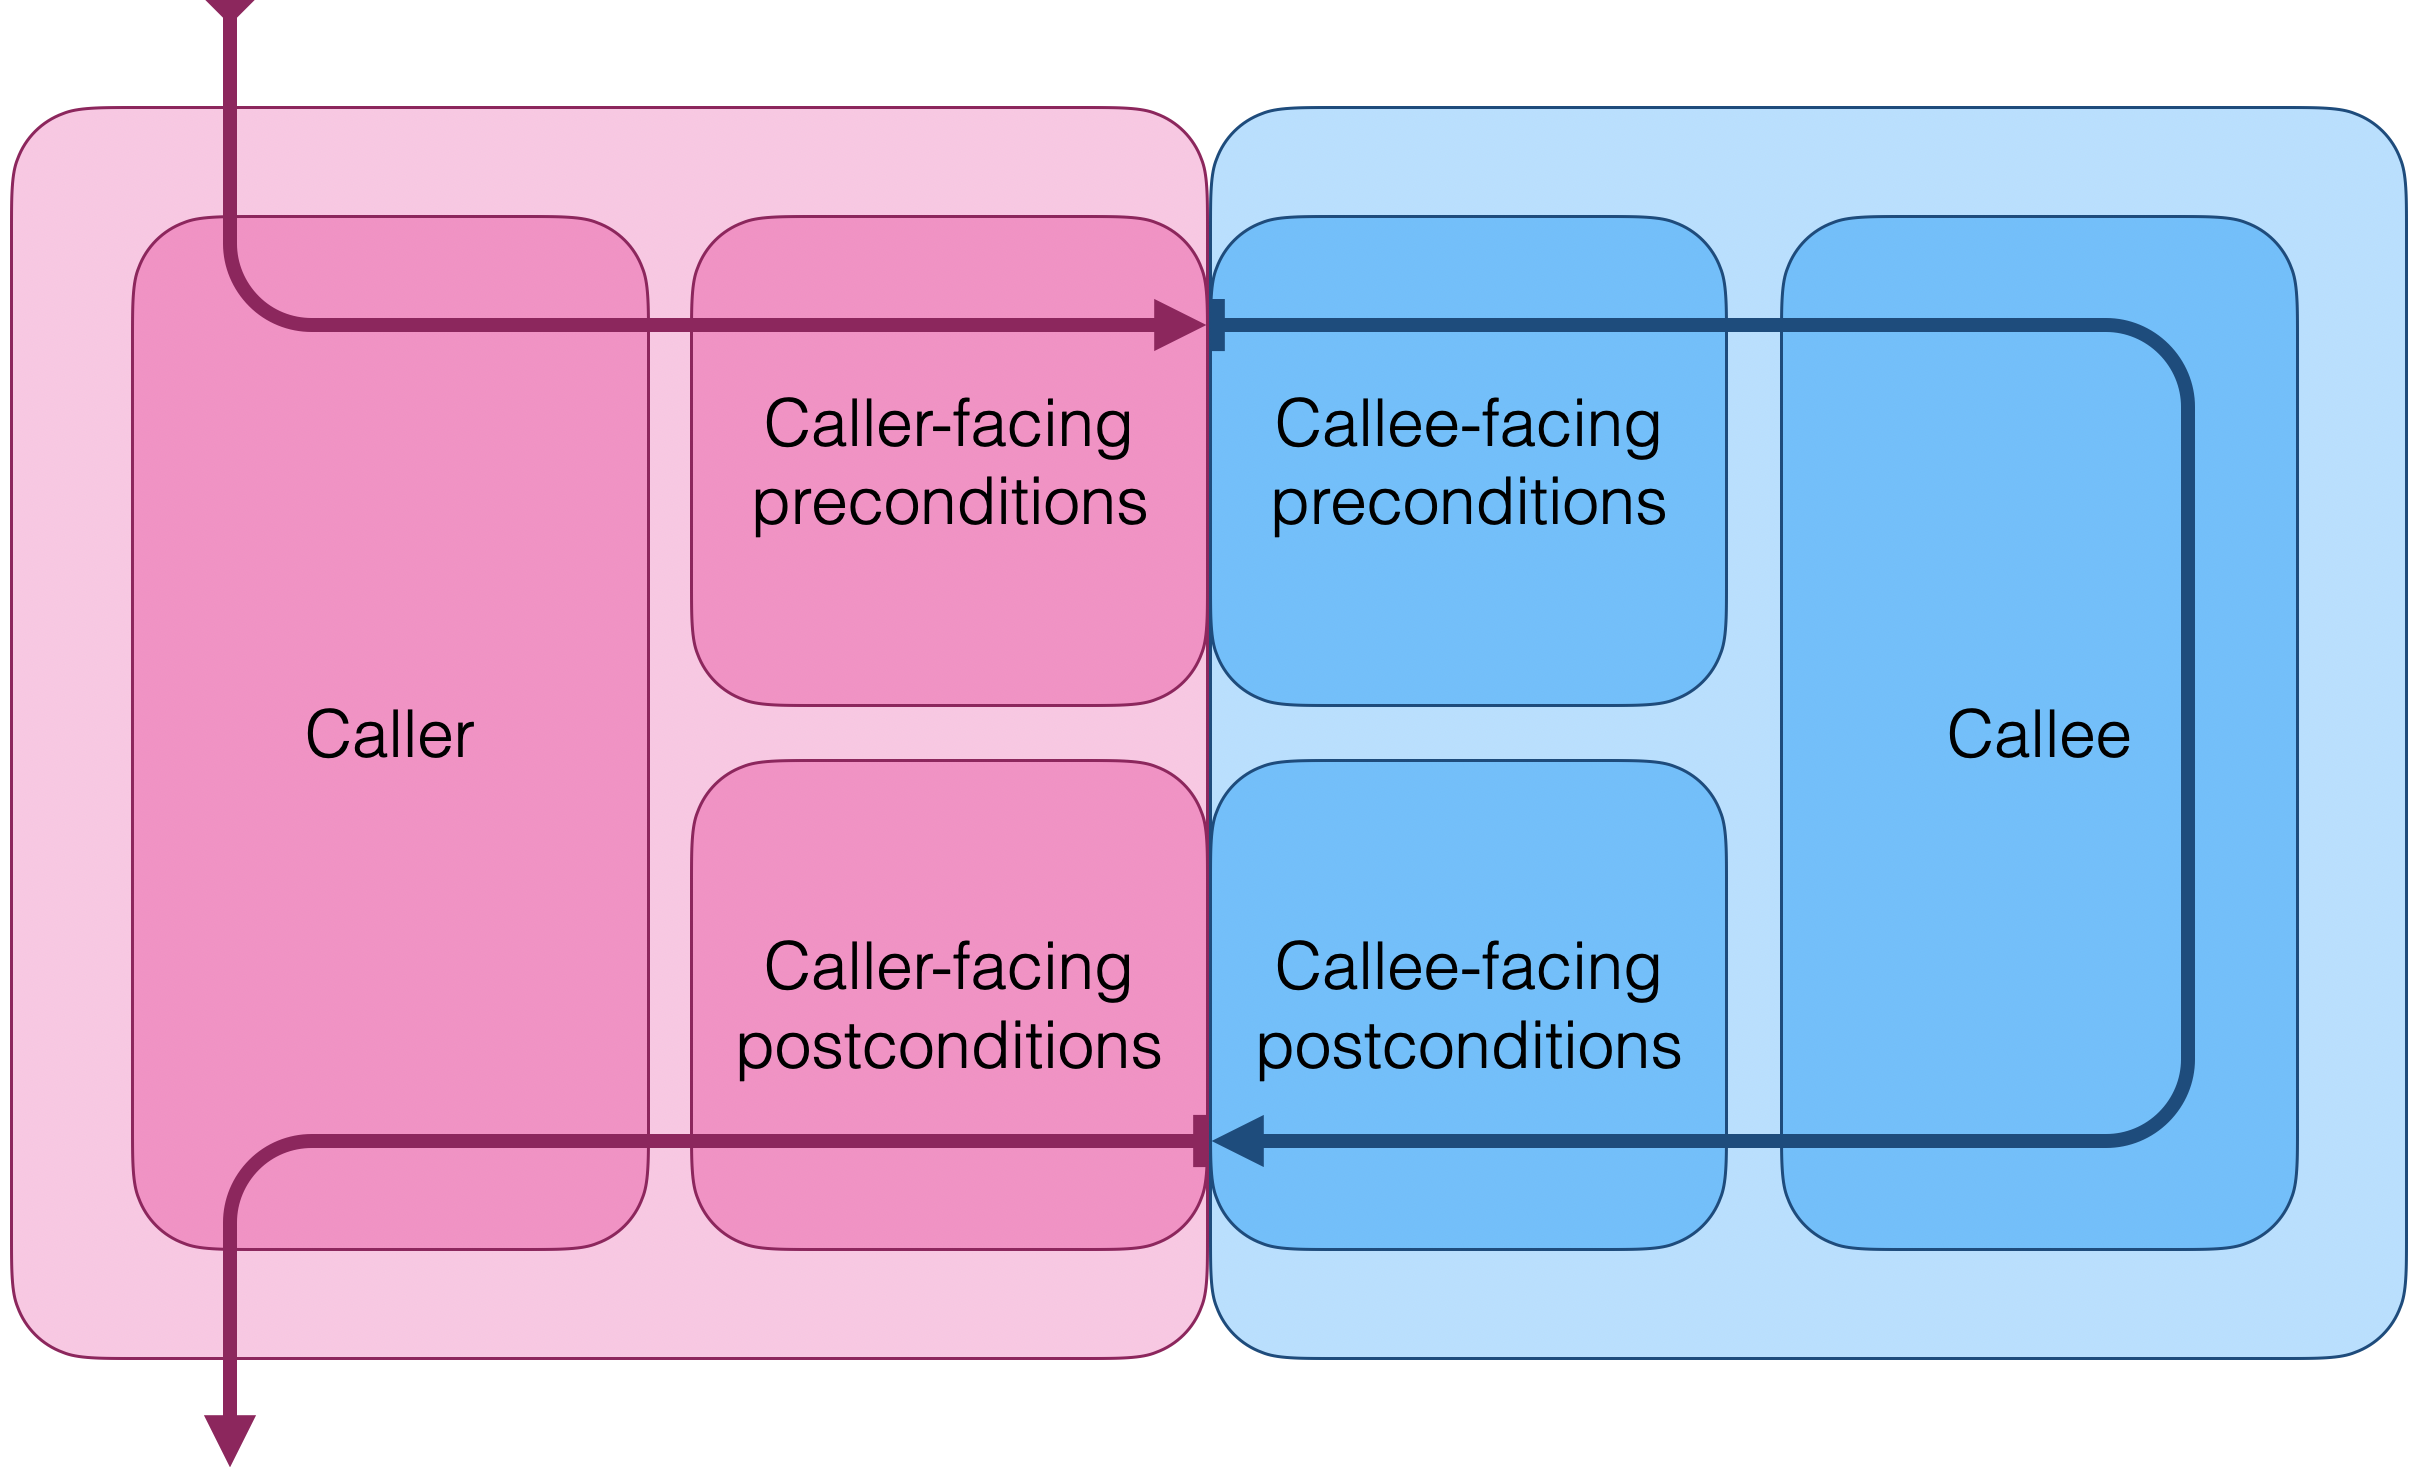
\includegraphics[scale=0.29]{images/D2900R9-callercallee}
\end{center}
\caption{Evaluation sequence of caller-facing and callee-facing function contract assertions in the Contracts MVP \cite{P2900R8}. In this model, \tcode{pre} and \tcode{post} on function pointers are caller-facing.}
\label{fig:callercallee}
\end{figure}
%~~~~~~~~~~~~~~~~~~~~~~~~~~~~~~~~~~~~~~~~~~~~~~~~~~~~~~~~~~~~~~~~~~~

This caller/callee model is used to specify contract assertions on virtual functions in the Contracts MVP. For virtual function calls, the caller-facing contract is that of the statically called function, while the callee-facing contract is that of the final overrider chosen by virtual dispatch. These are the only contracts checked in a virtual function call in \cite{P2900R8}; contracts on other classes in the same inheritance hierarchy are ignored (see also \ref{intermediate}).

This model can be equally applied to other kinds of indirect calls, including calls through a function pointer. For calls through a function pointer, the caller-facing assertions are those of the pointer (currently required to be empty by \cite{P2900R8} --- this restriction would be relaxed if we allow \tcode{pre} and \tcode{post} on function pointers), and the callee-facing assertions are those of the pointed-to function. 

\subsubsection{Substitution principle model}
\label{submodel}

In the caller/callee model, the contracts on the involved entities are completely independent from each other. An alternative model for indirect calls is the \emph{substitution principle} model that Eiffel, D, and Ada use for contracts on virtual functions. In this model, the involved contracts are not independent, but subject to constraints: the preconditions in an overriding function can only be wider than in the overridden function, and the postconditions can only be narrower. This model can also be applied to indirect calls through a function pointer: the preconditions on the pointed-to function can only be wider than on the pointer, and the postconditions can only be narrower.

For virtual function calls, SG21 found that this model was not an ideal fit for C++; rationale can be found in \cite{P3097R0}. Choosing this model for function pointers would therefore create a conceptual inconsistency in \cite{P2900R8}. It would also raise the question whether or how the substitution constraints should be enforced. We could follow the strategy chosen in Eiffel and D for virtual functions and enforce the constraints by OR-ing the involved precondition checks and AND-ing the postcondition checks during program execution. Alternatively, we could consider performing static subsumption proofs, which raises questions about the practical feasibility of such proofs.

%---------------------------------------------------------------------------------------------------------------------
\subsection{Intermediate contracts}
\label{intermediate}

Now, let us consider what happens when we assign the value of one function pointer to another function pointer. If both involved function pointers have the same contract assertion sequence, the situation seems obvious. This code should ``just work'' and the contract assertion sequence should be checked on calls through either pointer. But what if the two involved pointers have different contract assertions? Consider the following example (again, we could construct an analogous test case for initialising a function pointer variable, or passing a function address into a function taking a function pointer as a parameter):
\begin{codeblock}
int f(int i) /* may or may not have its own @pre@ and @post@ */;

int (*fptr1)(int i)
  pre (i % 2 == 0)      // must call with even integer
  post (r: r % 2 == 0); // guaranteed to return even integer

int (*fptr2)(int i)
  pre (i > 0)           // must call with positive integer
  post (r: r != 0);     // guaranteed to return non-zero integer

void test(int i) {
  fptr1 = f;
  fptr2 = fptr1;  // (1)
  fptr2(i);       // (2)
}
\end{codeblock}
Note that this example is different from that in \ref{ptrfundifferent} as there are now \emph{three} sets of contracts in play: that of \tcode{f}, that of \tcode{fptr1}, and that of \tcode{fptr2}. The question is whether the assignment at (1) should compile, and if it does, which assertions should be evaluated when the call at (2) is made. 

In the caller/callee model, the contract of \tcode{fptr2} is the caller-facing one, while the contract  of \tcode{f} is the callee-facing one. The contract of \tcode{fptr1} is neither caller-facing nor callee-facing; it is an \emph{intermediate contract}. We can thus rephrase the question: should intermediate contracts be well-formed, and if they are, should they be checked or not?

Note that there can be an unbounded amount of intermediate contracts:
\begin{codeblock}
void test(int i) {
  fptr1 = f;
  fptr2 = fptr1; 
  fptr3 = fptr2;
  // ...
  fptrn = fptrn_minus_1;
  fptrn(i);
}
\end{codeblock}
Note further that the set of intermediate contracts is not statically known and can depend on a runtime variable:
\begin{codeblock}
void test(bool b, int i) {
  // ...
  fptr3 = b ? fptr1 : fptr2;
  fptr3(i);
}
\end{codeblock}
Multiple design directions are theoretically possible which we discuss below. (To specify the semantics of the above case, we also need to specify whether and how contracts should propagate through expressions; this is discussed in section \ref{expr}).

%---------------------------------------------------------------------------------------------------------------------

\subsubsection{Intermediate contract must match caller-facing contracts}
\label{intermediatematch}

If we choose to enforce that the caller-facing contract assertion sequence (on the function pointer through which the call is made) and the callee-facing contract assertion sequence (on the function that ends up being called) are odr-identical, the only sensible choice seems to be that any intermediate contracts must be odr-identical as well, otherwise the program is ill-formed.

If we allow the caller-facing and the callee-facing contract to be different, we can still enforce that any intermediate contracts must be odr-identical to the calle-facing contract. This is possible as conservative choice. Again, we need to make sure that it is impossible to SFINAE on whether two entities have the same contract assertion sequence. 

\subsubsection{Implicitly drop intermediate contracts}
\label{implicitdrop}

Another option would be to make the above examples well-formed, but silently drop the intermediate contract, which would never be checked. 

Note that intermediate contracts can already arise with \cite{P2900R8} in the context of virtual functions. For example, consider a doubly-indirect call where a virtual function call happens through a pointer to member function:
\begin{codeblock}
struct Base {
  virtual void f() pre(a) post (b);
}

struct Derived {
  void f() override pre(c) post (d);
}

void test(Base& b) {
  b.f();  // (1)
  
  void (Base::*memptr)() = &Base::f;
  (b.*memptr)();  // (1)
}

int main() {
  Derived d;
  test(d);
}
\end{codeblock}
The above code is well-formed in \cite{P2900R8} today. For the call at (1), the caller-facing contract is that of \tcode{Base::f}, while the callee-facing is that of \tcode{Derived::f}. Both are checked; the evaluation sequence is \tcode{a} --- \tcode{c} --- \tcode{Derived::f} --- \tcode{d} --- \tcode{b}. However, for the call at (2), the caller-facing contact is that of the pointer to member function, which is currently required by \cite{P2900R8} to be empty (this restriction would be relaxed if we allow \tcode{pre} and \tcode{post} on function pointers). The evaluation sequence is therefore \tcode{c} --- \tcode{Derived::f} --- \tcode{d}; the contract of \tcode{Base::f} is an intermediate contract and is not checked.

The philosophy behind this model is that the only contracts we care about for correctness are the contract on the interface we are using to make the call and the contract on the function whose implementation we end up calling. Intermediate contracts are irrelevant for this particular call as they are neither part of the  interface that is being used nor part of the implementation that gets executed. We can adopt the same model for indirect calls through function pointers.

%---------------------------------------------------------------------------------------------------------------------

\subsubsection{Explicitly drop intermediate contracts}
\label{explicitdrop}

Alternatively, we could make it ill-formed if an intermediate contract was silently dropped --- to prevent this from happening unintentionally --- but allow such operations with an \emph{explicit} opt-in syntax that makes the intent of the developer clear:
\begin{codeblock}
void test(int i) {
  fptr1 = f;
  fptr2 = fptr1;                // Error: assignment would implicitly drop contract of \tcode{fptr1}
  fptr3 = drop_contract(fptr1)  // OK: contract of \tcode{fptr1} dropped explicitly
  fptr3(i)                      // checks contracts of \tcode{f} and \tcode{fptr3}, but not \tcode{fptr1}
}
\end{codeblock}
This approach seems compatible with the caller/callee model of the Contracts MVP, in which intermediate contracts are not checked, but recognises that for function pointers it can happen more easily that a contract ends up being dropped unintentionally than for virtual function hierarchies, as function pointers can be reassigned dynamically while virtual function hierarchies are known statically.

%---------------------------------------------------------------------------------------------------------------------

\subsubsection{Evaluate intermediate contracts}
\label{sticky}

Finally, we could consider breaking from the caller/callee model and check intermediate contracts. This would mean that the contract on a function pointer becomes ``sticky'':
\begin{codeblock}
bool a, b, c;
void f();

void (*fptr1)() pre (a) = f;
void (*fptr2)() pre (b) = fptr1;
void (*fptr3)() pre (c) = fptr2;

void test() {
  fptr3();  // checks \tcode{c}, then \tcode{b}, then \tcode{a}
}
\end{codeblock}
The contract would also ``stick'' when function pointers initialised with other function pointers or are passed as parameters into functions. This would enable use case \ref{usecase_inject}.

However, since the set of intermediate contracts is unbounded and not known statically, evaluating intermediate contracts leads to maintaining an arbitrarily long chain of contracts associated with each function pointer, perhaps through some kind of linked list structure that would have to be traversed at runtime for every function call through such a pointer. 

Similar to contracts on virtual functions, we could either consider all intermediate contracts to be independent from each other, or contemplate enforcing constraints on the relationship of all contracts in such a chain following the substitution principle model (see \ref{submodel}). Since the chain is not known statically, any such enforcement would have to happen at runtime.

%---------------------------------------------------------------------------------------------------------------------
\subsection{Expressions}
\label{expr}

The C++ Standard specifies that a function call is a postfix expression of function type or function pointer type followed by parentheses containing the arguments of the call. In all examples in this section so far, that postfix expression was an \emph{id-expression} directly naming a variable of function pointer type. In this simple case, the caller-facing contract is obviously known --- it is that on the declaration of the named pointer. However, a postfix expression of function pointer type can be arbitrarily complex, raising the question of whether and how the information about the contract of a function pointer should propagate through such expressions.

To illustrate the issue, consider the following example:
\begin{codeblock}
struct C {
  auto get_fptr() { return fptr; }
  
private:
  int (*fptr)(int x) pre (x > 0);  // (1)
};

void test(int i) {
  C c;
  c.get_fptr()(i);  // (2)
}
\end{codeblock}
The function pointer with a contract assertion sequence is defined as a private data member of a class at (1). The postfix expression at (2) is a prvalue that is itself the result of calling a member function that returns the function pointer. In order to insert the precondition check at (2), the contract check at (1) needs to propagate out of the class and through the expression.

We can make the example slightly more complicated by defining the contract on a typedef:
\begin{codeblock}
struct C {
  auto get_fptr() { return fptr; }
  
private:
  typedef int (*fptr_t)(int x) pre (x > 0);  // (1)
  fptr_t fptr;
};
\end{codeblock}
Now, if  we want to check the contract on the function pointer, the information from that typedef also needs to propagate through to the call site.

Even if we enforce that all contract assertions in a chain must be odr-identical, making the above examples ill-formed does not seem like a viable choice. If the postfix-expression of the function call is a prvalue expression such as \tcode{c.get_fptr()}, it is impossible for it to have its own contract assertions (see \ref{syntax_expr}); silently dropping the contract would likely be surprising to most users; therefore, the only option is to specify contract assertions on function pointers such that this information can propagate through the expression. Whether and how this can be achieved depends on the chosen specification strategy for contract assertions on function pointers; we will discuss three such strategies in Section~\ref{wherelive}.

Finally, consider an example where the contract depends on a dynamic variable:
\begin{codeblock}
// Function that returns pointer to function that only accepts positive numbers:
typedef int (*positive_fptr_t)(int i) pre(i > 0);
positive_fptr_t get_positive_fptr();

// Function that returns pointer to function that only accepts negative numbers:
typedef int (*negative_fptr_t)(int i) pre(i < 0);
negative_fptr_t get_negative_fptr();

void test(int i, bool b) {
  (b ? get_positive_fptr() : get_negative_fptr())(i);  // (1)
}
\end{codeblock}
It is unclear whether the above code should be ill-formed, or if not, which precondition should be checked on the function call at (1).

%---------------------------------------------------------------------------------------------------------------------

\subsection{Templates and type deduction}
\label{semantic_templates}

Finally, we need to consider the semantics of contract assertions on function pointers interacting with templates and type deduction. These semantics will determine whether we can enable use case \ref{usecase_templates}.

Consider storing a function pointer with contract assertions that is being used in a template such as \tcode{std::function} or a \tcode{std::vector}:
\begin{codeblock}
// Pointer to function that accepts only positive numbers:
typedef int (*positive_fptr_t)(int i) pre(i > 0);
positive_fptr_t positive_fptr = f;

void test(int i) {
  std::function<positive_fptr_t> positive_f = positive_fptr;
  positive_f(i);  // (1)
  
  std::vector<positive_fptr_t> positive_fs = {positive_fptr};
  positive_fs.front()(i);  // (2)
}
\end{codeblock}
Do we expect that the contract of \tcode{positive_fptr} will be checked in the calls at (1) and (2)?

What about cases where the function pointer is used to deduce the template argument:
\begin{codeblock}
void test(int i) {
  std::invoke(positive_fptr, i);  // (3)
}
\end{codeblock}
Do we expect that the contract of \tcode{positive_fptr} will be checked in the call at (3)?

Related to this is the question whether two function pointers that only differ in their contract assertion sequence should trigger two different template instantiations:
\begin{codeblock}
// Pointer to function that accepts only positive numbers:
typedef int (*positive_fptr_t)(int i) pre(i > 0);
positive_fptr_t positive_fptr = f;

// Pointer to function that accepts only negative numbers:
typedef int (*negative_fptr_t)(int i) pre(i < 0);
positive_fptr_t negative_fptr = g;

void test(int i) {
  std::invoke(positive_fptr, i);
  std::invoke(positive_fptr, i);  // same or different template instantiation?
}
\end{codeblock}
Furthermore, what should happen when we try to initialise a container with multiple function pointers that have different contracts:
\begin{codeblock}
std::vector v = {positive_fptr, negative_fptr};  // (4)
\end{codeblock}
Should class template argument deduction fail at (4), making the program ill-formed? If not, what contracts (if any) will be checked if either element of the vector is accessed and then called? What happens when we swap the two elements in the vector?

The answers to these questions are tightly linked to the specification strategy we choose for contract assertions on function pointers, which we discuss in the following section.

%%%%%%%%%%%%%%%%%%%%%%%%%%%%%%%%%%%%%%%%%%%%%
\section{Specification strategies}
\label{wherelive}


If we want to allow a function pointer to have its own sequence of function contract assertions, this information has to be stored \emph{somewhere}. The C++ language gives us three possible places: the sequence could be a part of the function pointer's type, it could be a part of its value, or it could be a property of a particular function pointer variable declaration. Each strategy enables a different set of semantic options (\ref{semantics}) to be implemented, and has different tradeoffs and limitations, which we discuss in this section.

\subsection{Contract as part of the type}
\label{type}

Our first option for specifying contract assertions on function pointers is to make them a part of the pointer's type. With this approach, two pointers that differ only in their sequence of contract assertions would have different types. Since the type of a function pointer is just ``pointer to some other type'', it follows that two \emph{functions} that differ only in their sequence of function contract assertions would have different types as well.

The type system approach would allow us to enforce that the caller-side contract or the callee-side contract must be the same (\ref{matching}), or allow them to be different (\ref{dropping}, \ref{adding}, \ref{ptrfundifferent}) by defining appropriate type conversion rules between these types. We could enforce that intermediate contracts must be the same as the caller-facing one (\ref{intermediatematch}), or drop intermediate contracts implicitly (\ref{implicitdrop}) or explicitly (\ref{explicitdrop}), all via type conversion rules; however, we could not build up a chain of ``sticky'' contracts (\ref{sticky}) through the type system unless the entire chain is known statically, which is not the case in general. 

Propagating contracts through arbitrary expressions (\ref{expr}) would happen automatically through the type system, since the contracts would be part of the type of the expression.

Finally, the type system approach would naturally allow contract assertions to propagate into templates (see \ref{semantic_templates}). 

However, the direct consequence of this design is that for any template that takes a function type as a template argument --- consider \tcode{std::sort}, \tcode{std::map}, \tcode{std::function}, etc. --- a difference in the function contract assertion sequence would trigger a separate template instantiation, even if the function type is otherwise the same, potentially significantly increasing the amount of distinct template instantiations in a program. 

Another consequence is that, if \tcode{pre} and \tcode{post} are part of the type,  then they must be part of name mangling. Since contract predicates can contain arbitrary C++ expressions, we would then need to find a way to mangle those too. At this point, contracts also become part of the ABI, which means that adding or changing the function contract assertions of a function can lead to an ABI break, which would violate an important design principle that \cite{P2900R8} is built on.

Apart from the ``no ABI break'' principle, a number of other design principles of \cite{P2900R8} would be violated by this direction, such as the Contracts Prime Directive and the No Caller-side Language Break principle.\footnote{ The \emph{No caller-side language break} principle stipulates that for any existing function \tcode{f}, if any function contract assertion is added to \tcode{f} and the definition of \tcode{f} still compiles after this addition, then any existing, correct usage of \tcode{f} should continue to compile and work correctly (as long as no contracts are being violated). However, if adding \tcode{pre} and \tcode{post} to a function can change its type, client code relying on that type might break in arbitrary ways.} Note that this is true regardless of whether we allow function pointers to have contract assertions distinct from the function they are pointing to and/or distinct from other pointers pointing to the same function (these options are discussed in Section~\ref{semantics}).

Making contracts part of the type system would raise a number of other questions. For example, what should \tcode{operator\&} do, and how should that will interact with type deduction? If we were to ever have \tcode{operator\&} changed to return ``pointer to function with that function's contract assertions'', this would break code like the following:
\begin{codeblock}
int f1() post (r: r > 0);
int f2() post (r: r < 0);

int x() {
  auto* f = &f2;   // pointer with assertion \tcode{post (r: r > 0)}
  if (rand()) {
    f = &f1;  // assigning to a function with a different, incompatible postcondition
  }
  f();  // violation if branch was taken! Certainly not the intent of the original code.
}
\end{codeblock}
Finally, how would making \tcode{pre} and \tcode{post} part of a function's type interact with overload resolution? Could we overload on different function contract assertions? Or would function contract assertions behave like \tcode{noexcept}, which is also part of the type system (since C++17) but cannot be overloaded on? Consider:
\begin{codeblock}
void f(int (*)(int x) pre(x == 0));  // Overload 1
void f(int (*)(int x) pre(x > 0));   // Overload 2 --- OK or ill-formed?

int r(int x) pre(x == 0);
int s(int x) pre(x > 0);
int t(int x);
int u(int x) pre(x == 0) pre(x == 0);
int v(const int x) pre(x == 0) post(x == 0);

f(&r);  // which f overload is called? Overload 1 seems likely
f(&s);  // which f overload is called? Overload 2 seems likely
f(&t);  // now what?
f(&u);  // ...and now?
f(&v);  // ...and now?
\end{codeblock}
Any proposal that makes contracts part of the type system needs to answer the questions above.

%---------------------------------------------------------------------------------------------------------------------

\subsection{Contract as part of the value}
\label{value}

Instead of making the sequence of contract assertions on a function pointer part of its type, we could encode the sequence in the pointer's value. To our knowledge, this strategy has not been considered by any previous contracts proposal.

With this approach, the contract assertion sequence of a function pointer would become a \emph{dynamic} property, unlike the contract assertion sequence of a function declaration. We would therefore be unable to statically enforce any relationship between caller-facing, intermediate, and callee-facing contracts, such as requirements that they be the same. However, we would be able to support arbitrary, dynamic chains of ``sticky'' contracts (\ref{sticky}). 

Propagating contracts through arbitrary expressions (\ref{expr}) would be possible but would happen dynamically during program execution, rather than statically as in the type system approach.

Generally, it seems inevitable that a value-based approach would incur some amount of runtime overhead when adding a contract assertion to a function pointer, regardless of whether the contract is actually ever checked, violating the \emph{Zero Overhead} principle from \cite{P2900R8}.

Below, we consider two different implementation strategies for value-based contracts.

\subsubsection{Thunks}

The obvious implementation approach to encoding contracts in the pointer value would be to generate a thunk that checks the contract assertions on the pointer and then calls the underlying function, and to store the address of that thunk in the pointer. This approach seems straightforward to implement, but has a number of consequences. First, directly inspecting the value of a pointer would not necessarily tell us whether it has a contract assertion sequence (as it just stores an address in either case). Second, if the pointer \emph{does} have a contract assertion sequence, the address that is the value of the pointer would no longer be equal to the address of the function that it is pointing to --- invalidating a property that the C++ Standard tries to guarantee.

In practice, there are already cases where this property is invalidated. For example, when using dynamic linking, loading a function \tcode{f} from a dynamic library and asking for the address of \tcode{f} will in practice yield two different answers inside and outside of that dynamic library. However, this new case would be different as we could get two different answers in the same translation unit, leading to surprising consequences.

For example, we might want to store pointers to functions in an array or vector (for example, to implement a user-level vtable or something similar), and look up certain functions in that vector by their address. If contract assertions on such pointers are part of their value, and implemented such that the pointers store the addresses of thunks rather than addresses of the actual functions, the function we are looking for may never be found, even if there is a pointer to it in the vector.

Moreover, the thunk approach requires devising a strategy for when to allocate and deallocate those thunks. Depending on the semantics we wish to support (allow or do not allow pointers to have contract assertions different from the function they point to and/or from other pointers that might point to that function, drop or retain intermediate contracts, etc.), we might be able to allocate all possible thunks statically, or we might have to do this dynamically, raising questions about how we would then deallocate them, given that there might not be a general way to keep track of the lifetime of those thunks.

%%%%%%%%%%%%%%%%%%%%%%%%%%%%%%%%%%%%%%%%%%%%%

\subsubsection{Wide pointers}

Instead of generating thunks, we can consider encoding contracts in the pointer value more directly by making function pointers with contract assertions wide pointers (a.k.a. ``fat'' pointers) that carry that information alongside the address of the pointed-to function. This approach would have some advantages over the thunk approach: we would be able to tell by inspecting the value of the pointer that it has a contract assertion sequence, and we could preserve the property that when that value is compared to an address, it could compare equal to the address of the function that the pointer points to. However, it would have the disadvantage that such an approach would change the binary representation of the pointer to one that is ABI-incompatible with function pointers today.

Note that the sequence of contract assertions on a function pointer can be arbitrarily long, and each contract assertion's predicate can be an arbitrarily long C++ expression. Therefore, even if we choose the wide pointer approach rather than the thunk approach, some part of that information necessarily has to live outside of the immediate object representation of the pointer, and be accessed via some form of indirection. The questions around allocating and deallocating storage for this information therefore apply equally to the wide pointer approach.

%---------------------------------------------------------------------------------------------------------------------

\subsection{Contract as property of the declaration}
\label{decl}

The third approach is to make the sequence of contract assertions on a function pointer a property of a particular pointer variable declaration, without it being a property of the pointer type or the pointer value.

This approach was used for the \tcode{noexcept}-ness of a function until C++17 (when \tcode{noexcept} was made part of the function type instead; see \cite{P0012R1} for rationale). It is still used in other parts of the language, for example for \tcode{alignas}:
\begin{codeblock}
int i = 0;
int j alignas(long) = 0;
\end{codeblock}
The two variables \tcode{i} and \tcode{j} have the same type, the same value (even the exact same bit representation of the value), and yet the compiler knows about the different alignment of variable \tcode{j}. The same approach is being used for many kinds of attributes and vendor-specific extensions (e.g., \tcode{__declspec}). This means that when using  \tcode{pre} and \tcode{post} on a function pointer, for example,
\begin{codeblock}
void test(int i) {
  int (*fptr)(int i) pre (i >= 0) = f;  // (1)
  fptr(i);  // (2)
}
\end{codeblock}
we could avoid the consequences of making  \tcode{pre} and \tcode{post} part of the pointer type or the pointer value. The compiler will see the contract on the declaration of \tcode{fptr} at (1) and will be able to generate the required checks around the call at (2), while adding \tcode{pre} and \tcode{post} will not have any effect on the ABI, will not break any client code, will not have additional runtime overhead, etc.

However, the downside of this approach is that with the rules of C++ today, it would be impossible to keep track of intermediate contracts and enforce any rules on them (\ref{intermediate}), or to propagate contracts through expressions (\ref{expr}). The reason for this is that in C++ today, so-called \emph{backchannel} information that is neither part of the type nor part of the value does not propagate through expressions, out of functions, etc. This includes information such as alignment, whether a variable was declared using a typedef, and --- with this specification strategy --- also the contract assertion sequence. Therefore, in all the code examples in \ref{expr}, the contract would just silently evaporate, as there is no language mechanism in C++ today to make the function call aware of it. This behaviour would likely be very unexpected to the user.

There is a possible solution to this problem. Existing compilers can --- and do --- propagate different kinds of backchannel information about ``attributed types'' in this manner today. Different compilers have made different implementation decisions in this area, which are not necessarily coherent; however, we could entertain introducing such a mechanism to the C++ Standard.

However, such a mechanism would not address another problem with this specification strategy, namely that there would still be no way for a contract assertion sequence to propagate into a template (\ref{semantic_templates}). Consider again two function pointers that only differ in their contract assertion sequence:
\begin{codeblock}
// Pointer to function that accepts only positive numbers:
typedef int (*positive_fptr_t)(int i) pre(i > 0);
positive_fptr_t positive_fptr = f;

// Pointer to function that accepts only negative numbers:
typedef int (*negative_fptr_t)(int i) pre(i < 0);
positive_fptr_t negative_fptr = g;

void test(int i) {
  std::invoke(positive_fptr, i);
  std::invoke(negative_fptr, i);  // same or different template instantiation?
}
\end{codeblock}
Since the contract assertions are not part of the type, the template arguments of \tcode{positive_fptr} and \tcode{negative_fptr} have the same type, and therefore must result in the same template instantiation. In other words, the template only sees the type of its template argument, not the backchannel information, and therefore generates the same code regardless of the contract assertion sequence. This must be so --- doing otherwise would be an ODR violation. Since the contract assertions are not part of the value either, there is simply no way for \tcode{std::invoke} to be aware of the contract assertion sequence on either pointer. We are currently not aware of any possible solution to this problem.

%%%%%%%%%%%%%%%%%%%%%%%%%%%%%%%%%%%%%%%%%%%%%

\section*{Acknowledgements}

Thanks to Gabriel Dos Reis, Lisa Lippincott, and Daveed Vandevoorde for the discussions that led to this paper; and to Joshua Berne, Ville Voutilainen, Peter Bindels, and Oliver Rosten for reviewing an earlier draft of it.

%%%%%%%%%%%%%%%%%%%%%%%%%%%%%%%%%%%%%%%%%%%%%

% Remove ToC entry for bibliography
\renewcommand{\addcontentsline}[3]{}% Make \addcontentsline a no-op to disable auto ToC entry

%\renewcommand{\bibname}{References}  % custom name for bibliography
\bibliographystyle{abstract}
\bibliography{ref}

%%%%%%%%%%%%%%%%%%%%%%%%%%%%%%%%%%%%%%%%%%%%%


\end{document}

